\chapter{Experiments}
\section{Motivation}
With the ultimate aim of leveraging equivariance for model-based RL. A series of Experiments were carried out, sequentially, to investigate how to exploit known symmetries in a model based environment.

Model-Based RL, is inherently more complex than Actor-Critic or Value based methods, as not only does a policy need to be learned, but also a model of the environment dynamics must also be learned.

Due to the increased complexity of Model based methods, and the benifit of implementing existing methods, while also providing a baseline for further experimentation a model free implementation was created.

\section{Baseline}
The baseline that was chosen was a proximal policy optimization agent from PureJaxRL,~\cite{lu2022discovered}. This baseline provides a training framework, that trains a single agent concurrently on multiple environments.

The Training regime is outlined below in pseudo code.
\begin{algorithm}
	\caption{PureJaxRL PPO Agent Training Structure}
	\begin{algorithmic}
		\State Initialize Agent: Actor-Critic $\pi_\theta$, $v_\phi$
		\State Initialize Replay Buffer: $\mathcal{D}$
		\For{Num Updates}
		\State Gain Experience For Num Timestep
		\State Store trajectories: $\mathcal{D}$.append($(S, A, S', R))$
		\State Calculate GAE Estimate From time steps
		\For{ Num Epochs}
		\State{ Split GAE Estimates into mini-batches}
		\State{ Mini-Batch SGD with Adam on $\pi_\theta, v_\phi$}
		\Comment{ See~\ref{alg:PPO} for Losses to optimize}
		\EndFor
		\EndFor
		\State Returns($\mathcal{D}$)

	\end{algorithmic}
\end{algorithm}

For the baseline, an MLP with two hidden layers of 64 units each were used in both the actor and the critic network. All the other training hyperparameters can be found in the appendix. To ensure that the learning curves were reproducible, 256 random seeds were averaged across. This ensures that the estimate of the baseline model is reliable.

\section{Equivariant Actor-Critics}
\subsection{CartPole}

To form an equivariant network to the group structure of CartPole the actor network must be equivariant to both the identity and inversion operator. In state space the inversion and identity operator $r, e$ are,
\begin{equation}
	\ell^\mathcal{S}_e =
	\begin{pmatrix}
		1 & 0 & 0 & 0 \\
		0 & 1 & 0 & 0 \\
		0 & 0 & 1 & 0 \\
		0 & 0 & 0 & 1 \\
	\end{pmatrix},
	\ell^\mathcal{S}_r =
	\begin{pmatrix}
		-1 & 0  & 0  & 0  \\
		0  & -1 & 0  & 0  \\
		0  & 0  & -1 & 0  \\
		0  & 0  & 0  & -1 \\
	\end{pmatrix}.
\end{equation}
Then the action space, the inversion and identity operator are,
\begin{equation}
	\ell^\mathcal{A}_e =
	\begin{pmatrix}
		1 & 0 \\
		0 & 1 \\
	\end{pmatrix},
	\ell^\mathcal{A}_r =
	\begin{pmatrix}
		0 & 1 \\
		1 & 0 \\
	\end{pmatrix}.
\end{equation}
Thus to parameterise an equivariant actor network, the network $\pi_\theta$ must satisfy,
\begin{equation}
	\pi_\theta(\ell^\mathcal{S}_e s) = \ell^\mathcal{A}_e \pi_\theta(s),
\end{equation}
\begin{equation}
	\pi_\theta(\ell^\mathcal{S}_r s) = \ell^\mathcal{A}_r \pi_\theta(s),
\end{equation}
Because the operation on the state space is equivariant to odd functions, the actor network, a simple solution is to use a network with only odd operations, ie $\tanh$ activation and no biases for all of the hidden representations. This ensures that the network is equivariant to the inversion operator. Then we use a group convolution layer to map between representations.

The full network can then be thought of as a composition of $f_\theta : \mathcal{S} \rightarrow \mathbb{R}^{|H|}$, an odd embedding MLP and $gc_\theta: \mathbb{R}^{|H|} \rightarrow \mathbb{R}^{\mathcal{A}}$ a group convolution layer that "lifts" the equivariance to the action space.
\begin{equation}
	\pi_\theta(s) = gc_\theta(f_\theta(s)).
\end{equation}
Then the non-trivial identity equivariance properties of the subnetworks are,
\begin{equation}
	f_\theta(-s) = -f_\theta(s),
\end{equation}
\begin{equation}
	gc_\theta(-x) =
	\begin{pmatrix}
		0 & 1 \\
		1 & 0 \\
	\end{pmatrix}
	gc_\theta(x),
\end{equation}
Where $gc_\theta(x) = [P(A=a_0), P(A=a_1)]$ describes the distribution over the binary actions of Cart-pole.


For all the experiments, we leave the critic to be a standard MLP, with no equivariance constraints. This may be a non-optimal setting in terms of performance, but it allows for a simple training loop.

With an equivariant actor critic network structure, the training procedure is the same as conventional PPO implementations, with the equivariant the actor network.

\subsection{CartPole Equivariant Actor Results}
\begin{figure}[H]
	\centering
	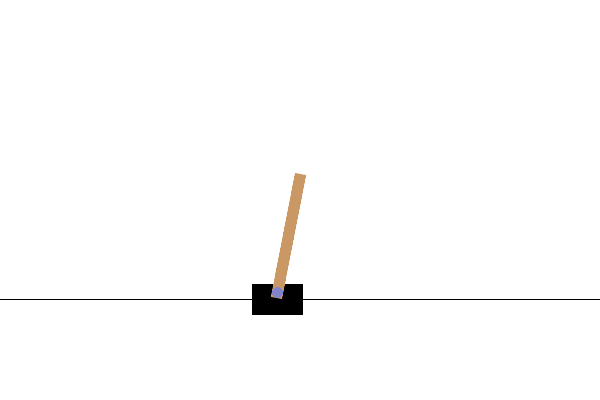
\includegraphics[width=0.8\textwidth]{Figures/cart_pole.png}
	\caption{CartPole Equivariant Actor Results} \label{fig:cartpole_equivariant_actor}
\end{figure}
